% Autor: Leonhard Segger, Alexander Neuwirth
% Datum: 2017-10-30
\documentclass[
	% Papierformat
	a4paper,
	% Schriftgröße (beliebige Größen mit „fontsize=Xpt“)
	12pt,
	% Schreibt die Papiergröße korrekt ins Ausgabedokument
	pagesize,
	% Sprache für z.B. Babel
	ngerman
]{scrartcl}

% Achtung: Die Reihenfolge der Pakete kann (leider) wichtig sein!
% Insbesondere sollten (so wie hier) babel, fontenc und inputenc (in dieser
% Reihenfolge) als Erstes und hyperref und cleveref (Reihenfolge auch hier
% beachten) als Letztes geladen werden!

\usepackage{tikz}
\usetikzlibrary{calc,patterns,angles,quotes} % loads some tikz extensions\usepackage{tikz}
\usetikzlibrary{babel}

% Silbentrennung etc.; Sprache wird durch Option bei \documentclass festgelegt
\usepackage{babel}
% Verwendung der Zeichentabelle T1 (Sonderzeichen etc.)
\usepackage[T1]{fontenc}
% Legt die Zeichenkodierung der Eingabedatei fest, z.B. UTF-8
\usepackage[utf8]{inputenc}
% Schriftart
\usepackage{lmodern}
% Zusätzliche Sonderzeichen
\usepackage{textcomp}

% Mathepaket (intlimits: Grenzen über/unter Integralzeichen)
\usepackage[intlimits]{amsmath}
% Ermöglicht die Nutzung von \SI{Zahl}{Einheit} u.a.
\usepackage{amssymb}
% mehr symbole plox
\usepackage{siunitx}
% Zum flexiblen Einbinden von Grafiken (\includegraphics)
\usepackage{graphicx}
% Abbildungen im Fließtext
\usepackage{wrapfig}
% Abbildungen nebeneinander (subfigure, subtable)
\usepackage{subcaption}
% Funktionen für Anführungszeichen
\usepackage{csquotes}
\MakeOuterQuote{"}
% Zitieren, Bibliografie
\usepackage[sorting=none]{biblatex}


% Zur Darstellung von Webadressen
\usepackage{url}
%chemische Formeln
\usepackage[version=4]{mhchem}
% siunitx: Deutsche Ausgabe, Messfehler getrennt mit ± ausgeben
\usepackage{floatrow}
\floatsetup[table]{capposition=top}
\usepackage{float}
% Verlinkt Textstellen im PDF-Dokument
\usepackage[unicode]{hyperref}
% "Schlaue" Referenzen (nach hyperref laden!)
\usepackage{cleveref}
\sisetup{
	locale=DE,
	separate-uncertainty
}
\bibliography{BA-C-04_SLM_27-05-2019_References}

\begin{document}

	\begin{titlepage}
		\centering
		{\scshape\LARGE Versuchsbericht zu \par}
		\vspace{1cm}
		{\scshape\huge Räumlicher LC-Modulator und diffraktive Optik \par}
		\vspace{2.5cm}
		{\LARGE Gruppe BA-C-04 \par}
		\vspace{0.5cm}

		{\large Alexander Neuwirth (E-Mail: a\_neuw01@wwu.de) \par}
		{\large Leonhard Segger (E-Mail: l\_segg03@uni-muenster.de) \par}
		\vfill

		durchgeführt am 27.05.2019\par
		betreut von\par
		{\large Milena Merkel}

		\vfill

		{\large \today\par}
	\end{titlepage}
	\tableofcontents
	\newpage

	\section{Kurzfassung}
	% Hypothese	und deren Ergebnis, wenn Hypothese ist, dass nur Theorie erfüllt, sagen: Erwartung: Theorie aus einführung (mit reflink) erfüllt
	% Ergebnisse, auch Zahlen, mindestens wenn's halbwegs Sinn ergibt
	% Was wurde gemacht
	% manche leute wollen Passiv oder "man", manche nicht

  \section{Theorie}
	% wdh. Texte
	% wdh. Besprechung

	\subsection{Gesetz von Malus}

	\subsection{Flüssigkristallzellen}
	%TODO ist ultra von dem anderen Versuch gecopypasted, aber das sollte ja wohl erlaubt sein.
	%TODO vlt mal in das alte Protokoll (MP5) schauen (kp, ob der das als pdf oder ausgedruckt wiedergegeben hat) und schauen, ob hier irgendwas falsch war.

	Flüssigkristalle zeichnen sich dadurch aus, dass sie mindestens unter bestimmten Bedingungen eine Orientierungsfernordnung, aber keine vollständige Positionsfernordnung, aufweisen, womit sie sich in letzterem Punkt von \enquote{gewöhnlichen} Kristallen unterscheiden.
	Positionsfernordnung bezeichnet hierbei eine Anordnung im Raum, die sich durch das periodische Fortsetzen einer Einheitszelle beschreiben lässt.
	Eine unvollständige Positionsfernordnung meint eine Periodizität in nur einer oder nur zwei Dimensionen.
	Orientierungsfernordnung meint, dass eine Vorzugsrichtung der Längsachsen der Moleküle des Flüssigkristalls existiert.
	Diese ist periodisch ortsabhängig oder konstant.
	Der Grad der Ordnung lässt sich als die Größe der durchschnittlichen Abweichung von der Vorzugsrichtung verstehen.

	Für die Herstellung von Flüssigkristallanzeigen wird ein Flüssigkristall in cholesterischer Phase verwendet. %TODO hier stand in der Anleitung immer "twisted nematic". Denke, das ist das gleiche.
	Dies meint, dass die Molekülachsen ebenenweise in die gleiche Richtung zeigen.
	Die Orientierung in den Ebenen ist dabei periodisch, da der Direktor (die Vorzugsachse) sich, wenn in Laufrichtung senkrecht zur Ebene betrachtet, mit konstanter Winkelgeschwindigkeit dreht und  eine Helixstruktur bildet, wenn das Ende des Direktorvektors im Raum verfolgt wird.

	\begin{figure}[H]
			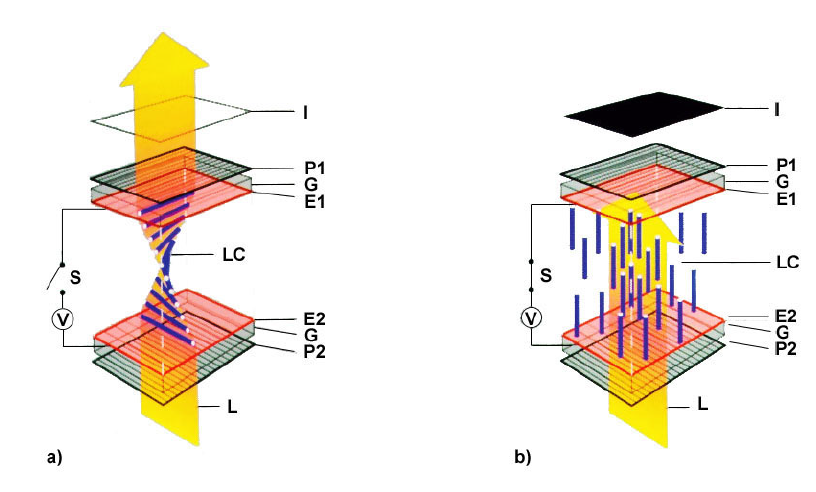
\includegraphics[width=1\linewidth]{img/displayHelix}
			\caption{
			Polarisationsrichtung in der Flüssigkristallanzeige. a) ohne angelegte Spannung. b) bei angelegter Spannung. E1, E2: Elektroden (ITO); G: Glasplatten; I: Lichtintensität; L: Lichtwelle; LC: Flüssigkristall;
P1, P2: Polarisatoren; S: Schalter, V: Spannungsquelle. \cite{displayHelix}
			}
			\label{fig_displayHelixBild}
	\end{figure}

	Dies erlaubt den Bau einer Flüssigkristallanzeige, da in einem Flüssigkristall in cholesterischer Mesophase die Polarisation des Lichtes, wenn es entlang besagter Laufrichtung einfällt, der Helixform des Direktors folgt.
	Wenn bekannt ist, mit welcher Ganghöhe (Länge der Helix bei einer Umdrehung des Direktors) der Kristall vorliegt, kann auf der Ausgangsseite des Displays linear polarisiertes Licht einen Polfilter passieren, wenn dieser zur Einfallsrichtung soweit gedreht ist, wie sich der Direktor über die Dicke des Flüssigkristalls im Display dreht.
	Häufig wird hierfür eine Vierteldrehung verwendet. Wie gleich deutlich wird, sind hier nur Drehungen um $\frac{\pi (2z+1)}{2}$ mit $z \in \mathbb{Z}$ praktikabel.
	Da für die lineare Polarisation des einfallenden Lichts ebenfalls ein Polfilter verwendet wird, ist eine solche Flüssigkristallanzeige bidirektional.
	Wenn jetzt im Flüssigkristall ein annähernd homogenes elektrisches Feld angelegt wird, richten sich die Molekülachsen statt nach der Helixstruktur mit zunehmender Feldstärke zunehmend eher nach dem Feld aus (vgl. \cref{fig_displayHelixBild}). %TODO , wenn es sich bei diesem um Dipole handelt.
	Dies verhindert, dass sich die Polarisation des Lichtes im Innern ändert, weshalb bei einer der oben genannten Drehungen zwischen den Durchlassrichtungen der Polarisationsfilter das Licht den zweiten Polarisationsfilter nicht passieren kann.
	Jetzt wird auch klar, warum nur die oben genannten Drehungen praktikabel sind:
	Die Polarisationsfilter müssen senkrecht zueinander stehen, damit im Falle von angelegter Spannung die Transmission minimal wird (vgl. Gesetz von Malus).

	Demnach ist eine spannungsgesteuerte Schaltung der Durchlässigkeit des Filters möglich und wenn hinter das Display eine Lichtquelle oder ein Spiegel gebracht wird, kann die Zelle als Pixel einer größeren Anzeige verwendet werden.
	Bei Farbdisplays werden Pixel aus drei Subpixeln zusammengesetzt, welche wiederum aus einer spannungsgesteuerten Flüssigkristallanzeige mit einem Farbfilter (Rot, Grün, Blau) bestehen. %TODO das ist für den Versuch recht egal...

	Flüssigkristalldisplays werden mit Wechselspannung betrieben, da eine Gleichspannung die elektrolytische Zersetzung des Flüssigkristalls zufolge hätte. %TODO wurde jetzt auch nirgendwo angesprochen.

\subsection{Doppelbrechung}
%TODO sie meinte, dass dies für die Polarisationsänderung in der Helix verantwortlich wäre. Sehe ich nicht so recht. sollte man aber erwähnen, wenn es true ist. ergibt sich irgendwie in dem Abschnitt 1.1.3 wegen der Jones-Rechnung.

	Flüssigkristalle weisen einen polarisationsabhängigen Brechungsindex auf, da die Molekülelektronen je nach Orientierung der Moleküle und Schwingungsrichtung sich gegenseitig unterschiedlich stark zum Schwingen anregen.
	Dies führt bei einem Strahl, der nicht bereits entweder senkrecht oder parallel zur optischen Achse polarisiert ist, zum Phänomen der Doppelbrechung.
	Der Strahl spaltet in zwei senkrecht zueinander polarisierte Strahlen auf.
	Diese Aufspaltung wird maximal, wenn der einfallende Strahl senkrecht zum Direktor steht.
	%Wenn der Flüssigkristall in einem keilförmigen Gefäß ist, behält der Strahl nach dem Austritt aus dem Kristall eine Winkelaufspaltung, weshalb in größerem Abstand die Aufspaltung einfacher gemessen werden kann (vgl. \cref{fig_keil}).
	%In einem plan-parallelen Aufbau würden die Strahlen nach dem Austritt aus dem Kristall wieder parallel verlaufen und die Ortsaufspaltung würde nicht mit dem Messabstand steigen.
  %Die Differenz der Brechungsindizes ist dabei direkt abhängig vom Ordnungsgrad, weshalb sie als ein Maß für diesen verwendet werden kann.

	Bei steigender Temperatur steigt die mittlere Abweichung der Molekülachsen vom Direktor und damit sinkt der Ordnungsgrad und die Differenz der Brechungsindizes.
	Ab einer bestimmten, materialabhängigen kritischen Temperatur verliert der Flüssigkristall seine Orientierungsfernordnung vollständig und das Phänomen der Doppelbrechung verschwindet.
	%TODO deswegen sind alle falschen Ergebnisse auf mangelnde Kühlung zurückzuführen.
	%TODO brauch man das?


	\subsection{Diffraktive Optische Elemente} %alles groß, weil Überschrift?
	%TODO Jones-Vektoren, Jones-Formalismus?

	Mithilfe einer Matrix aus Flüssigkristallzellen lässt sich ein räumlicher Lichtmodulator realisieren.
	%TODO 1.1.7 TN-LC-Zelle + Polarisator ergibt Amplitudenmodulation (und auch Phase)
	Polarisator, Mikrodisplay und Analysator sorgen in dafür, dass ein Phasenunterschied zwischen den Flüssigkristallzellen entsteht, der proportional zum eingestellten Grauwert ist.
	Dies ergibt sich aus der Betrachtung des Systems mittels des Jones-Formalismus.
	Durch einzelne Ansteuerung der Flüssigkristallzellen entsteht ein räumliche Lichtmodulation.

	%TODO Interferenz?

	\subsection{Kohärenz}
	Der signifikante Unterschied zwischen einem Laser und einer Glimmlampe besteht in der Fähigkeit zur Interferenz.
	Die Lichtwellen, die den Laser verlassen haben eine feste Phasenbeziehung, weshalb nach Trennung des Strahls Interferenz zwischen beiden Teilstrahlen zu beobachten ist.

	Bei der qualitativen Beschreibung der Interferenzfähigkeit unterscheidet man zwischen räumlicher und zeitlicher Kohärenz.
	Zeitliche Kohärenz kann über Autokorrelation mittels des Michelson-Interferometers gemessen werden.
	Die Kohärenzlänge ist definiert durch den Abstand (optische Wegdifferenz), der die Länge eines Arms des Interferometers vom Interferenzmaximum wegbewegt werden kann, bevor die durch die Interferenz erzeugte Autokorrelationsfunktion nicht mehr über $1/\text{e}$ steigt.
	Die Kohärenzlänge ergibt sich aus der Monochromatizität des Lichts, da sich bei perfekt monochromatischem Licht die Phasenbeziehung über keine Entfernung ändert.
	Die räumliche Kohärenz kann mittels eines Doppelspaltexperiments (oder des Young-Interferometers) gemessen werden, da sie die Phasenbeziehung innerhalb einer Wellenfront beschreibt und der Doppelspalt Interfernz zwischen unterschiedlichen Teilen der Wellenfront realisiert.

	%TODO Fraunhofer-Beugung?
	%TODO Was erwarten wir bei Doppelspalt, gitter, einzelspalt, etc.
	%TODO Was sind DOEs?

	\section{Methoden}
	% Bilder von der Website klauen
	% einer will Präsens
	%TODO irgendwo hier nen Bild hin?

	\subsection{Überprüfung des Gesetzes von Malus}
	Um das Gesetz von Malus zu überprüfen, wird das Licht eines He-Ne-Lasers durch einen Analysator geschickt und dann mit einer Linse auf ein Intensitätsmessgerät geschickt. %TODO He-Ne können wir nicht confirmen, aber ist schon ziemlich safe.
	Hierbei wird vermutet, dass der Laser bereits linear polarisiertes Licht erzeugt.
	Der Analysator wird in \SI{10}{\degree}-Schritten um \SI{360}{\degree} rotiert.

	\subsection{Einstellung der Eingangspolarisation}
	Der im Folgenden verwendete LC-Modulator weist einen von der Eingangspolarisation abhängigen Kontrast auf.
	Der maximale Kontrast soll bei einer Eingangspolarisation von \SI{-45}{\degree} bzw. \SI{-135}{\degree} liegen.
	Um diese Eingangspolarisation zu erreichen wird ein Analysator in den Strahlengang gebracht und auf \SI{-135}{\degree} eingestellt.
	Dann wird der Laser rotiert, bis die gemessene Intensität maximal ist.
	Sobald diese Position gefunden ist, wird zwischen Laser und Analysator der LC-Modulator eingebaut, der Strahl kollimiert und mit einer Kamera das sich ergebende Bild aufgenommen.
	Auf dem LC-Modulator wird ein horizontal geteiltes Bild eingestellt (eine Hälfte Weiß, eine Schwarz).
	Dann wird der Analysator um je \SI{90}{\degree} gedreht und jeweils ein Kamerabild aufgenommen, um zu zeigen, dass bei der gewählten Eingangspolarisation der Konstrast tatsächlich maximal ist. %TODO man sollte hier streng genommen bei einem Winkel von 90deg ein invertiertes Bild verwenden. not sure why, haben wir aber nicht gemacht.

	Zusätzlich wird der Kontrast gemessen, indem ein komplett weißes (schwarzes) Bild verwendet wird und mit einem Intensitätsmessgerät nach Fokussierung durch eine Linse die Intensität in der Fokusebene gemessen wird.

	\subsection{Bestimmung der Pixelgröße}
		\subsubsection*{Variante 1}
		Um die Pixelgröße des LC-Modulators zu bestimmen, wird ein weißes Bild mit einem 200x200 Pixel großen schwarzen Quadrat in der Mitte auf den Modulator gegeben.
		In den Strahlengang wird der LC-Modulator und im Abstand der Brennweite eine Linse dahinter gestellt, hinter der wieder im Abstand der Brennweite ein Schirm aufgestellt wird.
		Auf dem Schirm wird die Größe des Quadrats mit einem Lineal gemessen. %TODO waren wir hier wirklich nicht mit dem Modulator im Fokus? Hatten wir hier überhaupt einen Polarisator, an dem wir hätten falsch messen können?
		\subsubsection*{Variante 2}
		Da die Pixel des LC-Modulators elektronische Strukturen zur Ansteuerung benötigen, bilden sie ein periodisches Gitter. %TODO sagte sie nicht noch irgendwas, woraus die Pixel bestehen würden?
		Aufgrund dessen ergibt sich in der Fokusebene das Beugungsbild eines Gitters.
		Es wird der Abstand zweier höherer Ordnungen mit einem Lineal gemessen und hieraus Gitterkonstante und somit Piselgröße bestimmt.


	\subsection{Zusammenhang zwischen Grauwert und Polarisationszustand}

		Es wird auf dem LC-Modulator ein einfarbiges Bild angezeigt. %TODO streng genommen Weiß/Schwarz keine Farben, wenn man pedantisch ist...
		In der Fokusebene wird die Intensität gemessen und bei sechs verschiedenen Grauwerten des Bildes jeweils das Maximum der Intensität in Abhängigkeit vom Analysatorwinkel gesucht. %TODO ups. hier sollte man sich dann auch maximale und minimale Intensität notieren. Ich sehe aber nicht, wofür man das brauchen sollte.



	\subsection{Intensitätsverteilung in den Beugungsordnungen des unadressierten Displays} %TODO hier habe ich jetzt komplett den Titel übernommen
	Die Linse wird entfernt und stattdessen der Laser mittels der Linse am Laser auf einen Abstand von etwa \SI{80}{\centi \meter} fokussiert. %TODO haben wir da einen exakten Wert?
	Es wird in horizontaler und vertikaler Richtung die Intensität der ersten elf Ordnungen gemessen. %TODO hier haben wir halt horziontal weniger. kp, ob man das hier oder unten erwähnen sollten.

	\subsection{Beugungsbilder verschiedener DOEs}
		Der Laser wird wieder kolminiert und eine Linse nach dem Analysator zur Fokussierung verwendet.
		Es wird nacheinander ein Einzelspalt, zwei verschiedene Doppelspalte und ein Gitter als DOE für den LC-Modulator eingestellt.
		Dann wird mit einer Kamera in der Fokusebene jeweils das Beugungsbild aufgenommen.
		Für ein Gitter wird der Strahl mit der Linse am Laser (unter Entfernung der anderen Linse) auf einen Abstand von etwa \SI{1,23}{m} fokussiert und die Intensität des nullten und ersten Beugungsmaximums gemessen.

	\subsection{Brennweite eines Fresnel-Linsen-DOEs}
		Es wird als Bild eine Fresnel-Zonenplatte eingestellt.
		Dann wird für vier verschiedene Linsenphasen mithilfe der Kamera der Fokus des Laserstrahls gesucht, um die Abhängigkeit zu bestimmen.

	\subsection{Verschiedene DOEs als Hologramme}
		Es wird wieder der kolminierte Laserstrahl mit Fokussierung nach dem Analysator mit der Kamera in der Fokusebene verwendet.
		Es wird das Bild eines Schriftzugs und einiger geschachtelter Rechtecke am LC-Modulator eingestellt. %TODO Originalbilder hier oder später zum direkten Vergleich?
		Mit der Kamera wird jeweils ein Bild aufgenommen.
		Zuletzt wird auf der einen Hälfte des DOEs das Bild von geschachtelten Rechtecken und auf der anderen Hälft von geschachtelten Kreisen dargestellt und ein Kamerabild aufgenommen.



	\section{Ergebnisse und Diskussion}
	% Allgemeine Beobachtungen
	% Einflüsse von veränderten Parametern auf Messung
		\subsection*{Unsicherheiten}
	% Berechung nach Aufgabenstellung
	%TODO Unsicherheiten

	Folgende Unsicherheiten werden angenommen:
	\begin{description}
		\item[Winkel:] analog, somit Dreiecksverteilung, $u(\phi)=\frac{\SI{2}{\degree}}{2\sqrt{6}}=\SI{0.4}{\degree}$.
		\item[Intensität:] digital, wobei die letzte Ziffer häufig schwankte, $u(I)=\frac{\SI{0.01}{mW}}{2\sqrt{3}}=\SI{0.003}{mW}=\SI{0.003}{}$ a.u.
		\item[Brennweite:] Da keine Unsicherheit auf der Linse angegeben ist, wird einen Rechteckverteilung für die letzte Ziffer abgeschätzt $u(f)=\frac{\SI{1}{cm}}{2\sqrt{3}}= \SI{0.3}{cm}$
		\item[Abstand:] analog, Dreiecksverteilung $u(d)=\frac{\SI{0.1}{cm}}{2\sqrt{6}}= \SI{0.02}{cm}$
	\end{description}
		\subsection{Überprüfung des Gesetzes von Malus}\label{ss_malus}
		%4.1.1
		%TODO plotten und cos^2 reinfitten
		%TODO Kontrast angeben (vmtl halt einfach Differenz der Intensitäten minmax)
		In \cref{fig_malus} wurde die gemessenen Intensitäten gegen den Winkel des Polarisators aufgetragen.
		Es wurde ein Fit nach dem Gesetzt von Malus durchgeführt mit:
		\begin{equation}
			I = (I_\text{max}-I_\text{min})\cos^2(\phi\omega-\theta) +I_\text{min}
		\end{equation}
		Der Kontrast lässt sich quantitativ mit \cref{eq_kontrast} beschreiben.
		\begin{equation}
			\label{eq_kontrast}
			C = \frac{I_\text{max}-I_\text{min}}{I_\text{max}+I_\text{min}}= \input{res/malus_kontrast}
		\end{equation}

	\begin{figure}[H]
			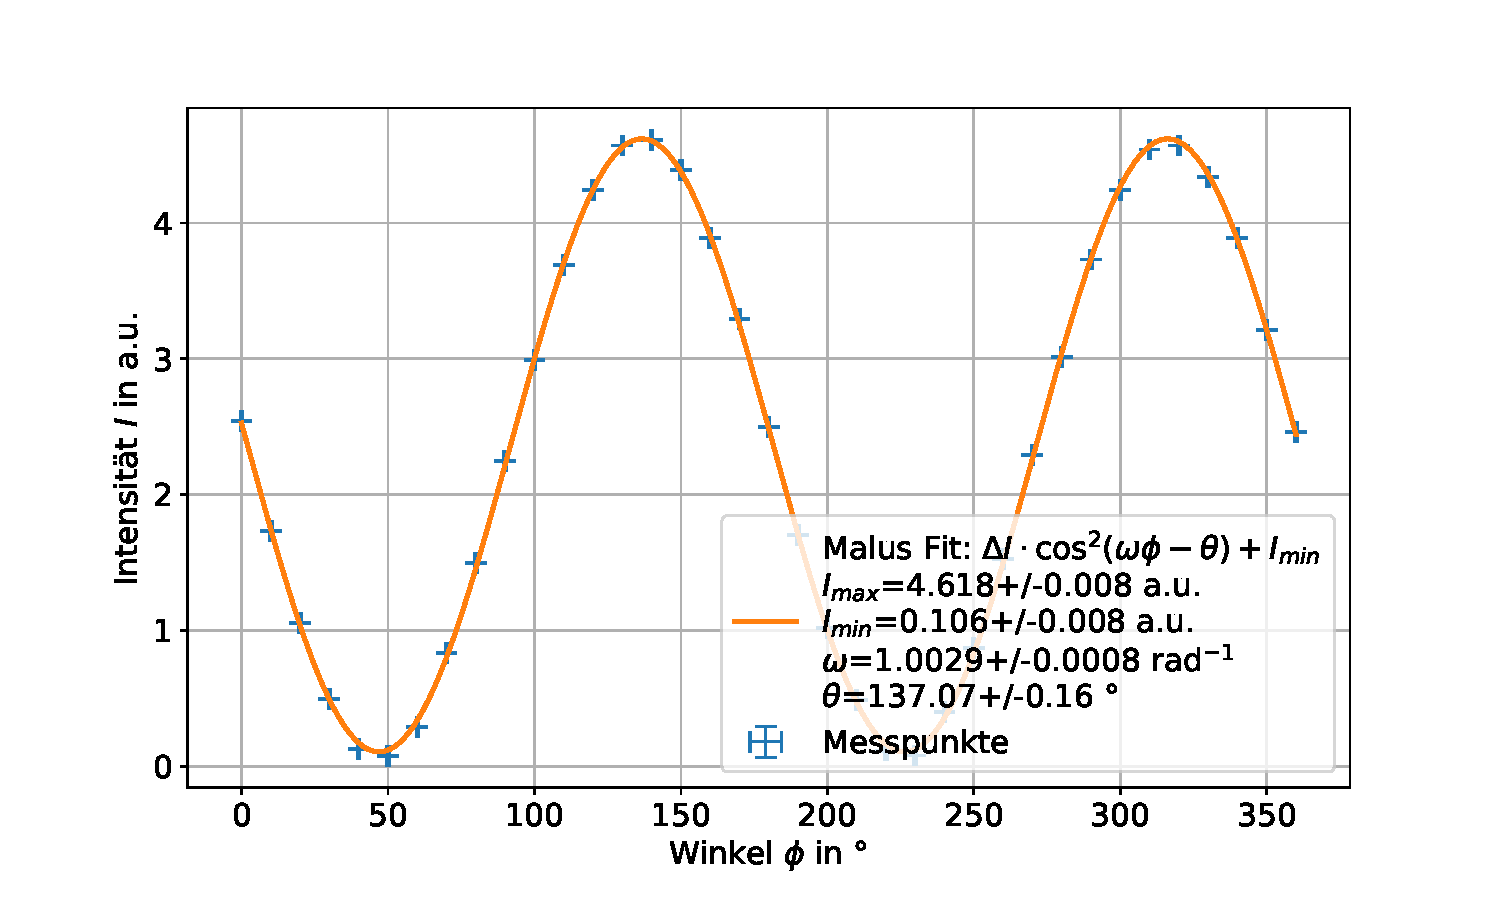
\includegraphics[width=0.8\linewidth]{img/malus}
			\caption{
			Messung der Intensität in Abhängigkeit vom Winkel des Polarisators.
			Die gelbe Funktion ist eine Fit nach dem Gesetzt von Malus.
			}
			\label{fig_malus}
	\end{figure}




			\subsubsection*{Diskussion}
			%TODO Frequenz = 1 passt, Maximum passt+- mit Augenmaß von 142
			%TODO im Kontext von Malus diskutieren

			%TODO Kreise sind gefourierte Punkte (1xgefouriert)
			%TODO Dreck ist auf Kamera (theoretisch auf Laser, aber dann wärs vmtl nicht so scharf)
			%TODO Wellen sind da, weil das gefourierte halt nicht bis ins unendliche geht

		\subsection{Einstellung der Eingangspolarisation}
		%4.1.2
		%TODO Kontrast für die vier Analysatorwinkel aus den Bildern (da steht explizit qualitativ. Reicht also wohl die Bilder zu printen und zu sagen: "Sieht man ja, wa?")
		%TODO Intensitätsmessung 0 und 255 für horizontally divided
		In \cref{fig_divscreen} sind für vier Analysatorwinkel im Abstand von \SI{45}{\degree} die Kamerabilder aufgeführt.
		Hierbei wurde auf den LC-Modulator ein \textit{Horizontally Divided Screen} gegeben.
		\begin{figure}[H]
        \centering
        \begin{subfigure}[b]{0.475\textwidth}
            \centering
            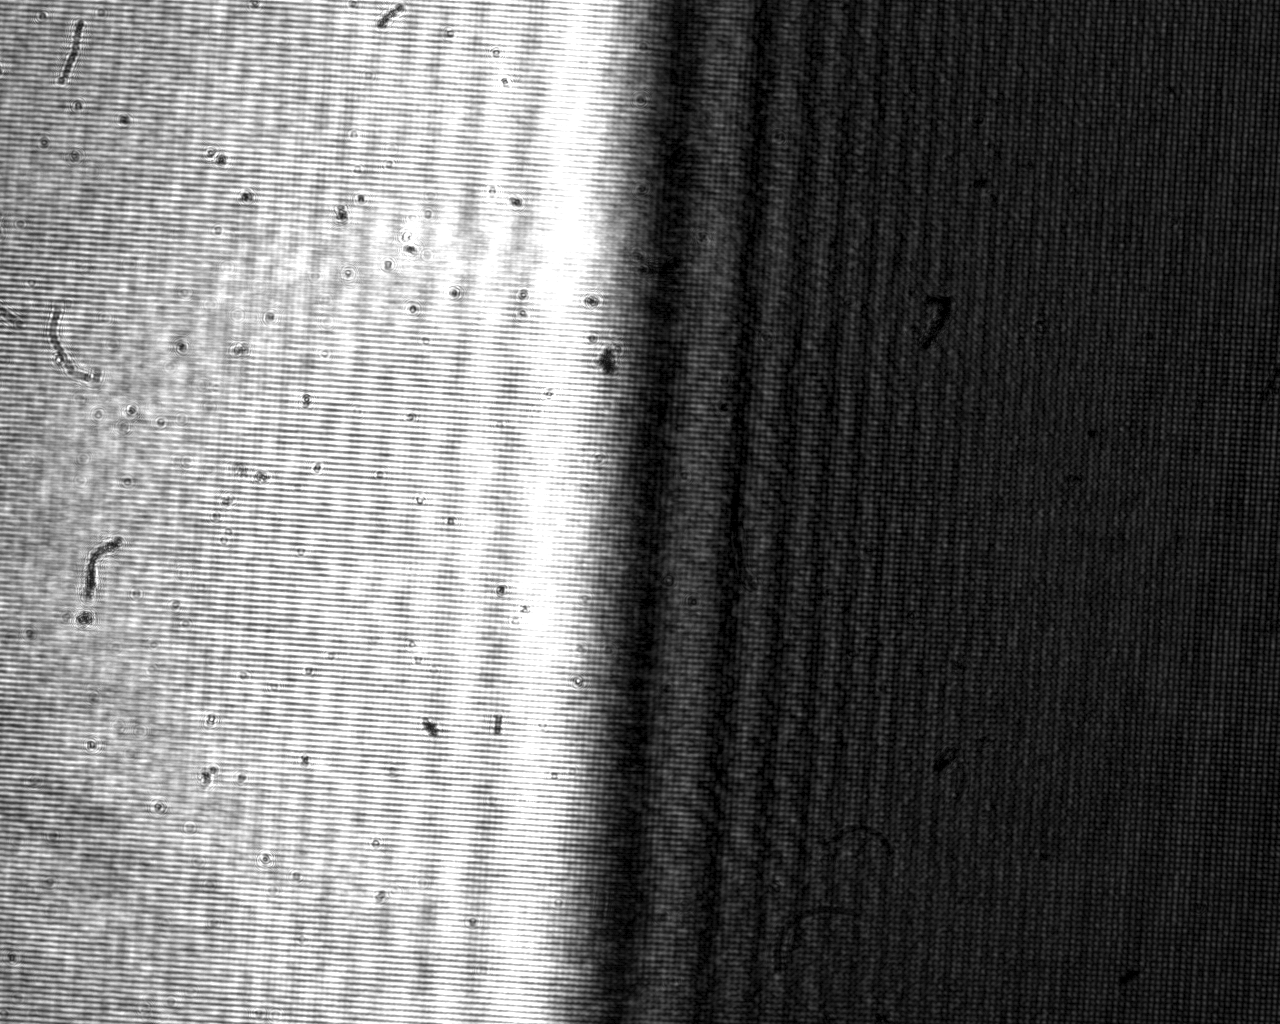
\includegraphics[width=\textwidth]{raw/dividedscreen_0_deg}
            \caption%
            {$\alpha=\SI{0}{\degree}$}
            \label{fig_divscreen_0}
        \end{subfigure}
        \hfill
        \begin{subfigure}[b]{0.475\textwidth}
            \centering
            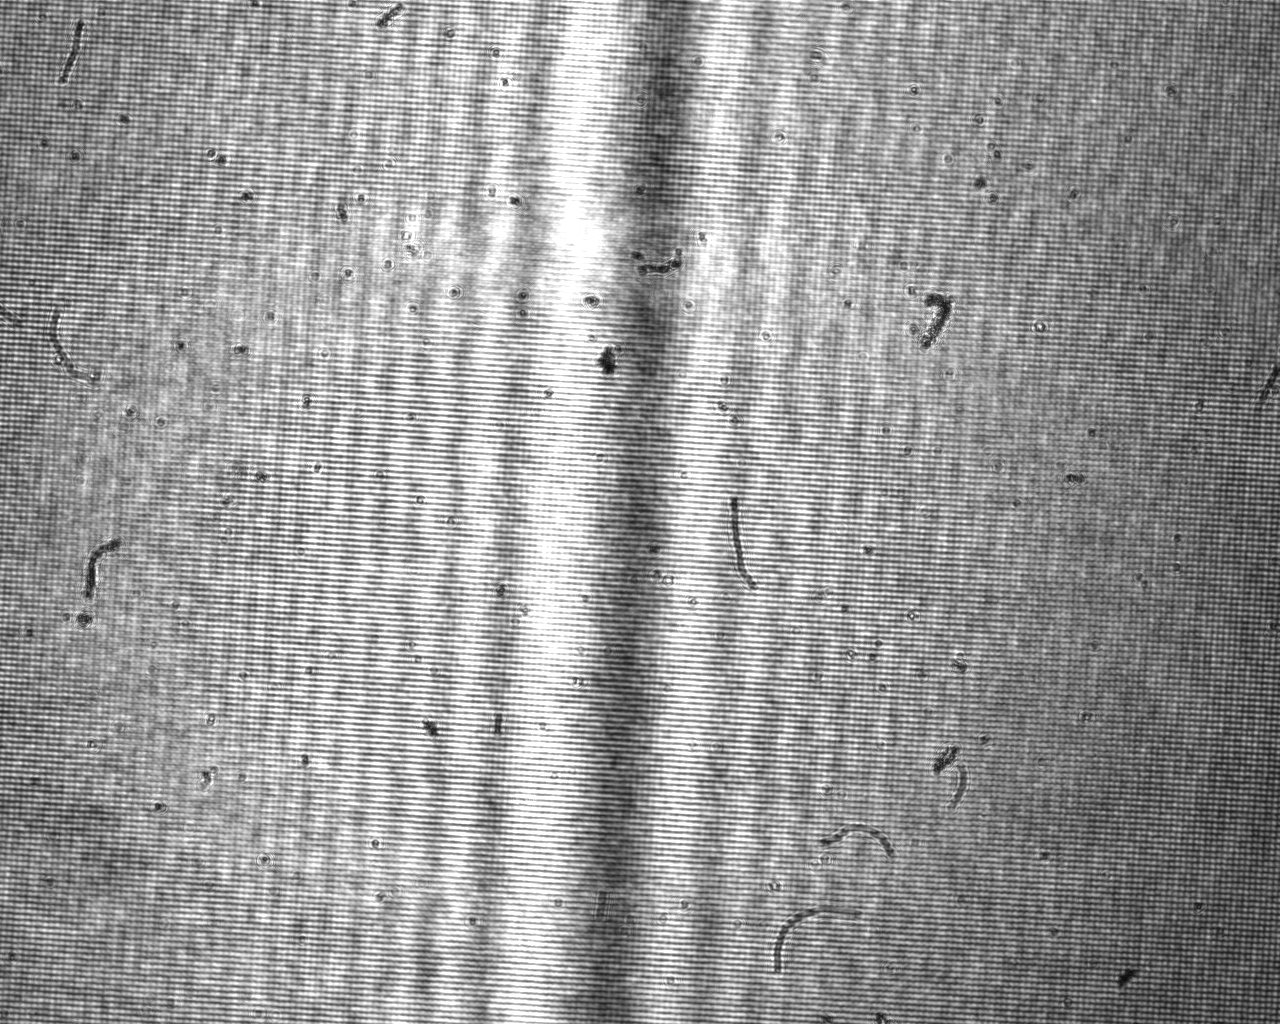
\includegraphics[width=\textwidth]{raw/dividedscreen_45_deg}
            \caption[]%
            {$\alpha=\SI{45}{\degree}$}
            \label{fig_divscreen_45}
        \end{subfigure}
        \vskip\baselineskip
        \begin{subfigure}[b]{0.475\textwidth}
            \centering
            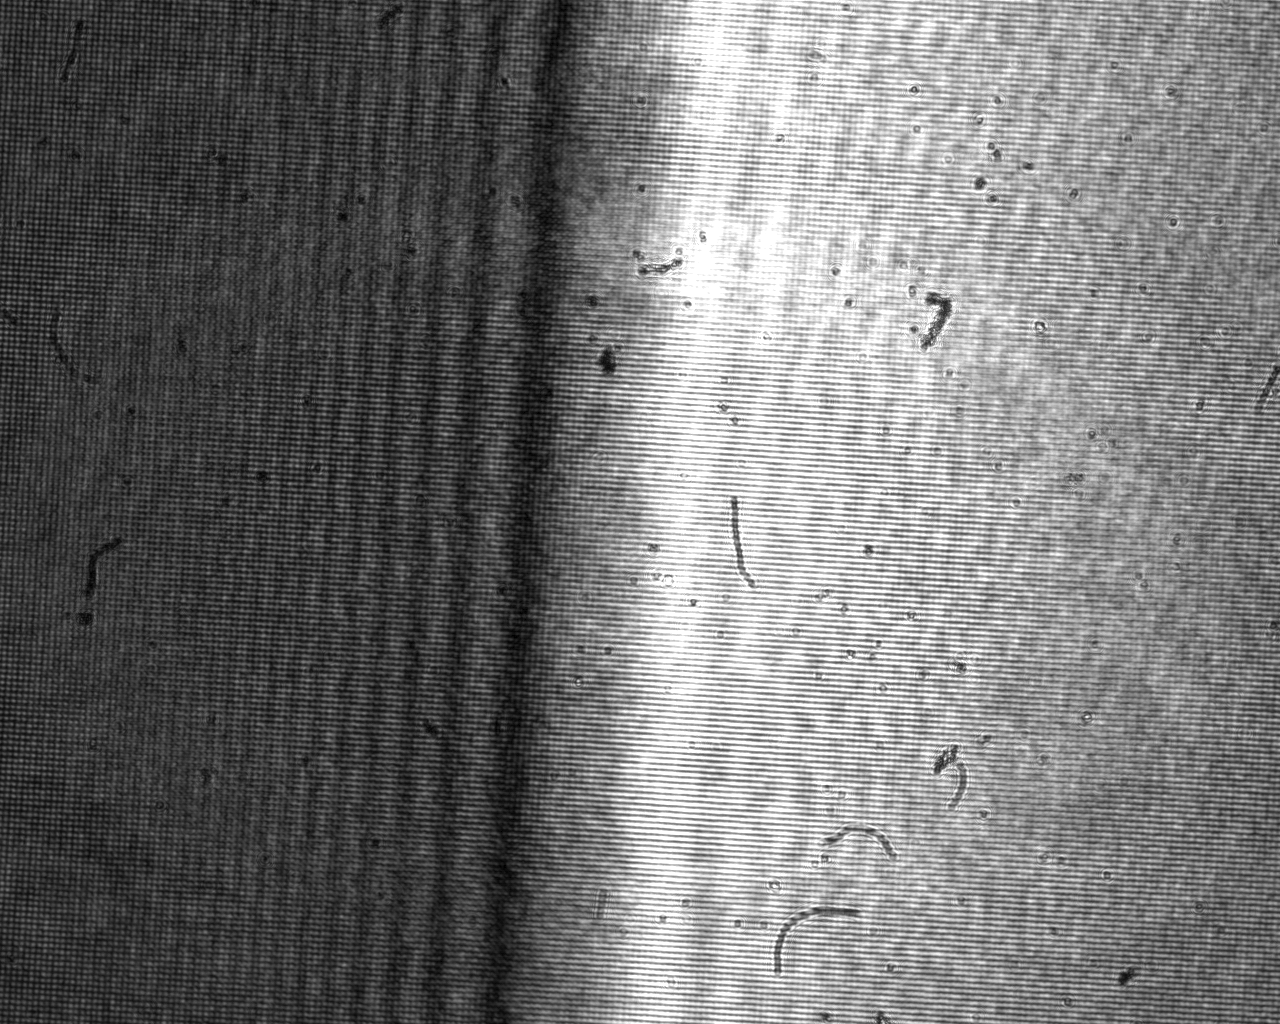
\includegraphics[width=\textwidth]{raw/dividedscreen_90_deg}
            \caption[]%
            {$\alpha=\SI{90}{\degree}$}
            \label{fig_divscreen_90}
        \end{subfigure}
        \quad
        \begin{subfigure}[b]{0.475\textwidth}
            \centering
            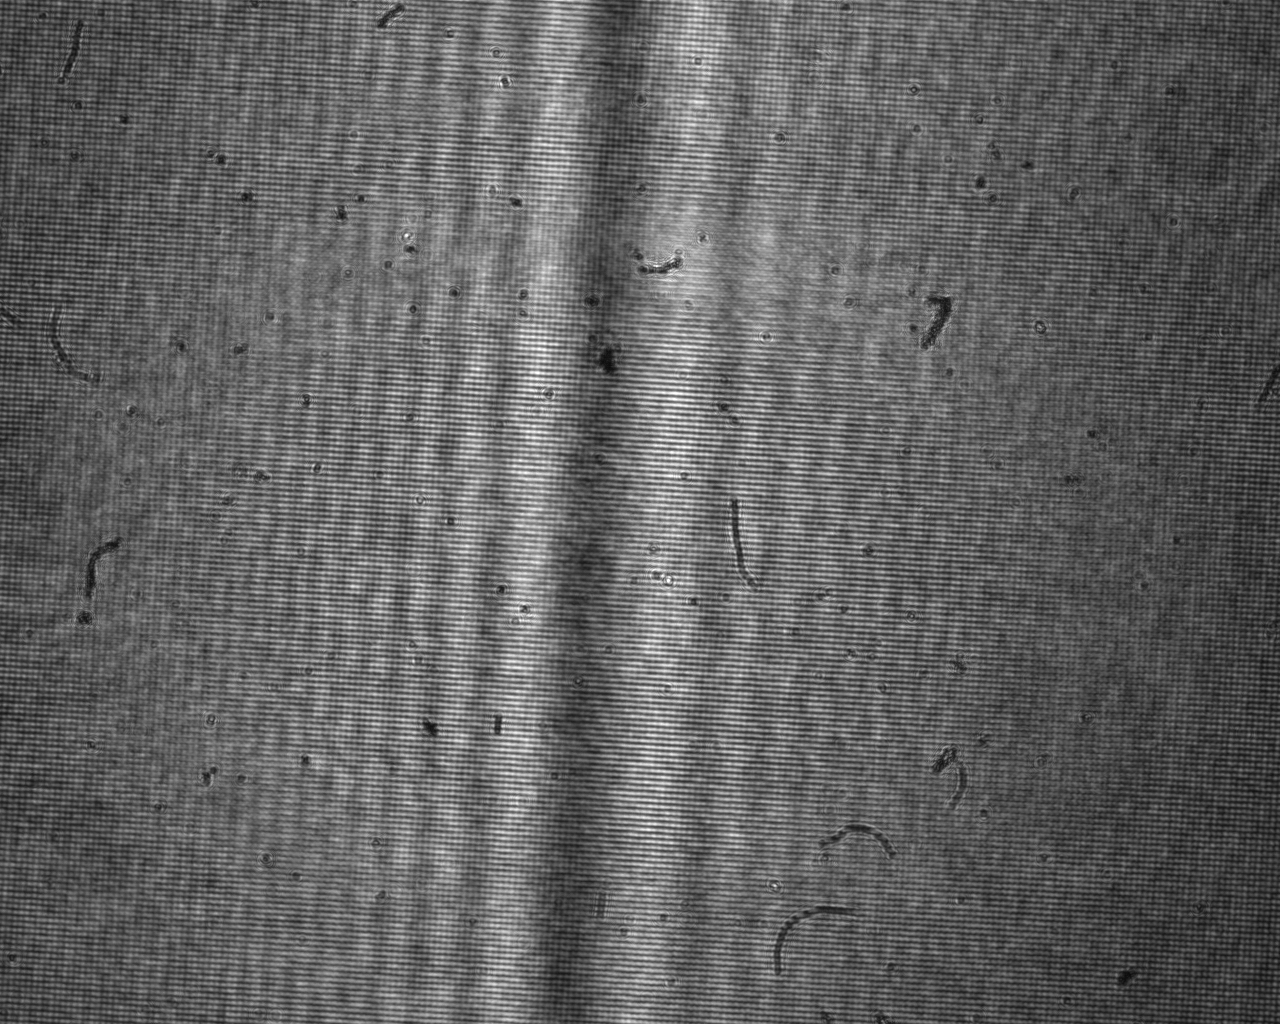
\includegraphics[width=\textwidth]{raw/dividedscreen_135_deg}
            \caption[]%
            {$\alpha=\SI{135}{\degree}$}
            \label{fig_divscreen_135}
        \end{subfigure}
        \caption%
        {Kameraaufnahmen für verschiedene Analysatorwinkel $\alpha$ mit einem \textit{Horizontally Divided Screen} auf dem LC-Modulator.}
        \label{fig_divscreen}
    \end{figure}


		Die Bestimmung des Kontrast erfolgt analog zu \cref{eq_kontrast} in \cref{ss_malus}, jedoch mit  den gemessenen intensitäten $I_\text{max}=\input{res/intens_max}$ und $I_\text{min}=\input{res/intens_min}$, respektiv für einen weißen und schwarzen \textit{Blank Screen}, sodass sich ein Kontrast von $C=\input{res/intens_kontrast}$ ergibt.
			\subsubsection*{Diskussion}
			%TODO qualitativ: ist tatsächlich deutlich anders
			%TODO Optimierung des Kontrastes bei LC-Modulator als Amplitudenmodulator beschreiben und erklären

		\subsection{Bestimmung der Pixelgröße} %: Achtung, ich habe hier die beiden zusammengechoben und den dazwischen dahinter geschoben
		%TODO Konsistenz mit Pixelabstand vs Pixelgröße
		Die verwendete Linse hat eine Brennweite $f$ von \SI{20+-0.3}{cm} und die Wellenlänge $\lambda$ des HeNe-Lasers beträgt \SI{632.8}{nm}.
			\subsubsection*{Variante 1}
			%4.1.3
			%TODO ausrechnen und Messungenauigkeit abschätzen

			Die Größe $G$ des \SI{200}{}x\SI{200}{} Pixel Quadrats auf dem LC-Display lässt sich aus Bildgröße $B$, Bildweite $b$ und Brennweite $f$ mit \cref{eq_fokus} berechnen. %TODO x mathmode?
			Der Pixelabstand $p$ ergibt sich aus dem Quotienten von $G$ und Höhe des Quadrats in Pixeln.
			Für die Unsicherheit $u$ der Höhe des Quadrats in Pixeln wird einen Rechteckverteilung  von $u = \frac{\SI{10}{px}}{2\sqrt{3}}= \SI{3}{px}$ verwendet, da Bilder von 800x600 Pixel auf den LC-Modulator mit 824x624 Pixel skaliert werden und auch der Rahmen des Bildprogramms mit an den LC-Modulator übertragen wird.
			Die Messungen sowie der resultierende Pixelabstand $p$ sind in \cref{tb_pixel} tabelliert.
			\begin{equation}
				\label{eq_fokus}
				G = \frac{B}{b/f-1}
			\end{equation}

\begin{table}[H]
		\centering
		\begin{tabular}{ c | c | c | c }
			 Bildweite $b/\si{cm}$ & Bildgröße $B/\si{cm}$ & Größe $G/\si{cm}$ & Pixelabstand $p/\si{\mu m}$ \\ \hline
			 \input{res/tb_pixel}
		\end{tabular}
		\caption{
		Gemessene Bildweite $b$, Bildgröße $B$ und berechnete Größe $G$, Pixelgröße $p$.
		}
		\label{tb_pixel}
\end{table}
			\subsubsection*{Variante 2}
			%4.2.1
			%TODO ausrechnen

			Für Beugung an einem Gitter mit der Gitterkonstanten $g$ gilt für das $m$. Maximum:
			\begin{equation}
				g \cdot \sin{\alpha} = m \lambda
			\end{equation}
			Für kleines $\alpha$ gilt $\alpha\approx\sin{\alpha}\approx\tan{\alpha}=\frac{d}{2f}$, wobei $d$ der Abstand zwei Maxima gleicher Ordnung $m$  zueinander ist und somit:
			\begin{equation}
				g = \frac{2m\lambda f}{d}
			\end{equation}


\begin{table}[H]
		\centering
		\begin{tabular}{ c | c | c }
			 Ordnung $m$ & Abstand $d/\si{cm}$ & Pixelabstand $p/\si{\mu m}$ \\ \hline
			 \input{res/tb_gitter}
		\end{tabular}
		\caption{
		Gemessene Abstand $d$, Bildgröße $B$ und berechnete Pixelgröße $p$.
		}
		\label{tb_gitter}
\end{table}
			\subsubsection*{Diskussion}
			%TODO beide Werte mit Materialbeschreibung vergleichen. aus der Anleitung von dem SLM?

		\subsection{Zusammenhang zwischen Grauwert und Polarisationszustand}
		%4.1.4
		%TODO plotten
					\subsubsection*{Diskussion}
			%TODO Zusammenhang zwischen Grauwert und Drehwinkel erklären. Wie ist die Ausrichtung der Flüssigkristalle im LC-Modulator ohne Angelegte Spannung-> helix obv.

		\subsection{Intensitätsverteilung in den Beugungsordnungen des unadressierten Displays}
		%4.2.2
		%TODO Trennung horzontale und vertikale Strukturen
		%TODO Intensität bei 1-10 plotten
		%TODO duty cycle bestimmen: Verhältnis transparenter Teil / lichtundurchlässiger Teil anhand der Intensitätsmodulation
		%TODO Füllfaktor (Verhältnis transparent / gesamt) abschätzen: pixel quadratisch. -> ??? Dann ergibt sich der Füllfaktor doch instant aus dem duty cycle. Das klingt aber sehr anders gemeint in 4.2.2


		Der Tastgrad $c$ ist definiert als das Verhältnis einer Impulsdauer $\tau$ zur Periodendauer $T$, also $c=\tau/T$.
		Übertragen auf die Transparenz der Pixel ist $c=t/g$.
		Wobei $t$ die Ausdehnung des transparenten und $g$ des gesamten Pixels beschreibt.


		Für Gitter gilt, dass das Produkt aus Periodizität im Realraum $r$ und reziproken Raum $P$ konstant ist, $rP=\text{const.}$.
		Im Experiment sind zwei Gitter simultan vorhanden, welche beide eine Fouriertransformation zur Folge haben.
		Eines welches die Pixelgröße definiert und eines welches der Steuerelektronik entstammt.
		Somit folgt:
		\begin{equation}
			gG =tT = \text{const.}
		\end{equation}
		Wobei $G$ und $T$ die respektiven Periodizitäten im reziproken Raum sind und es folgt, dass sich das Transparentsverhältnis $c=t/g=G/T$ im reziproken Raum als Verhältnis der Frequenzen widerspiegelt.

		In \cref{fig_sinc1} sind die Intensitäten der vertikalen Maxima aufgetragen.
		Maxima sind deutlich bei $m=\{0,4,7,9\}$ und Minima bei $m=\{3,6,8\}$.
		Der geringe Abstand zwischen den Maxima $\{7,9\}$ und dem Minimum $\{8\}$, lässt darauf folgern, dass im Bereich nahe der 0. Ordnung ein weiteres Minimum nicht aufgelöst werden konnte.
		Und es lässt sich das Verhältnis der Frequenzen durch das Verhältnis der Maxima beschreiben $c_v=4/9$.
		Analog stellt man in \cref{fig_sinc2} fest, dass $c_h=2/9$ beträgt und ebenfalls das erste Minimum nicht aufgelöst werden konnte.
		Mit einer Betrachtung der Unsicherheit welche durch eine Rechteckverteilung der Breite 1 am Punkt $m=9$ abgeschätzt und es folgt mit $m=\SI{9+-0.3}{}$ Tastgrade von $c_v=\SI{0.444(15)}{}$ und $c_v=\SI{0.222(7)}{}$.


		Als grobe Schätzung ergibt sich der Füllfaktor aus dem Produkt der Tastgrade:
		\begin{equation}
			\text{FF} \approx c_v c_h =\SI{9.9+-0.7}{\percent}
		\end{equation}


\begin{figure}[H]
			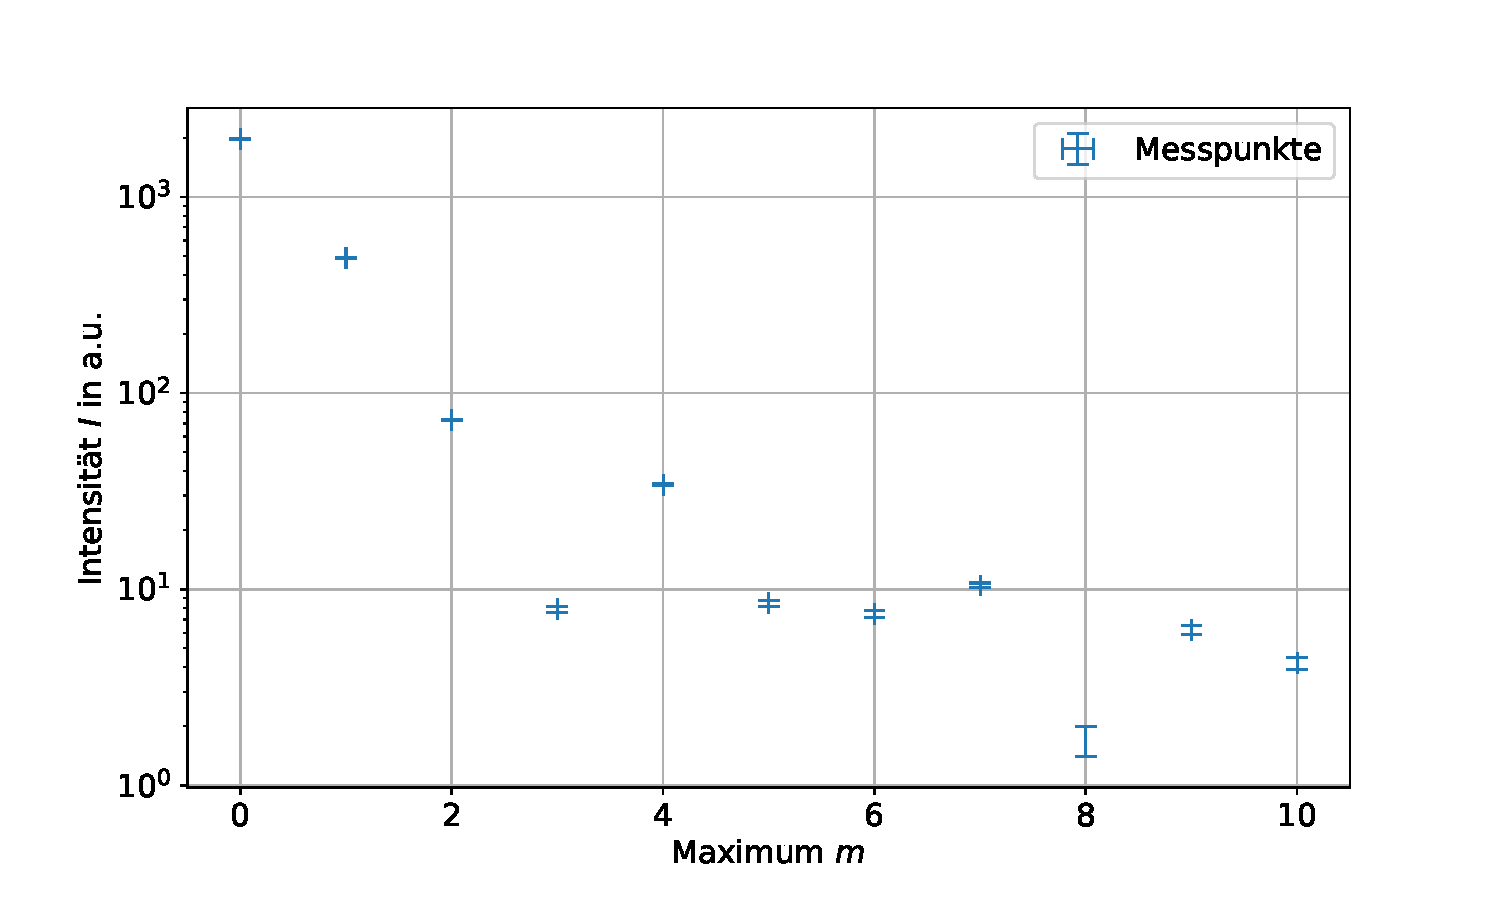
\includegraphics[width=0.8\linewidth]{img/sinc1}
			\caption{
			Messung der Intensität in Maxima der Gitterbeugung in vertikaler Richtung.
			}
			\label{fig_sinc1}
	\end{figure}

\begin{figure}[H]
			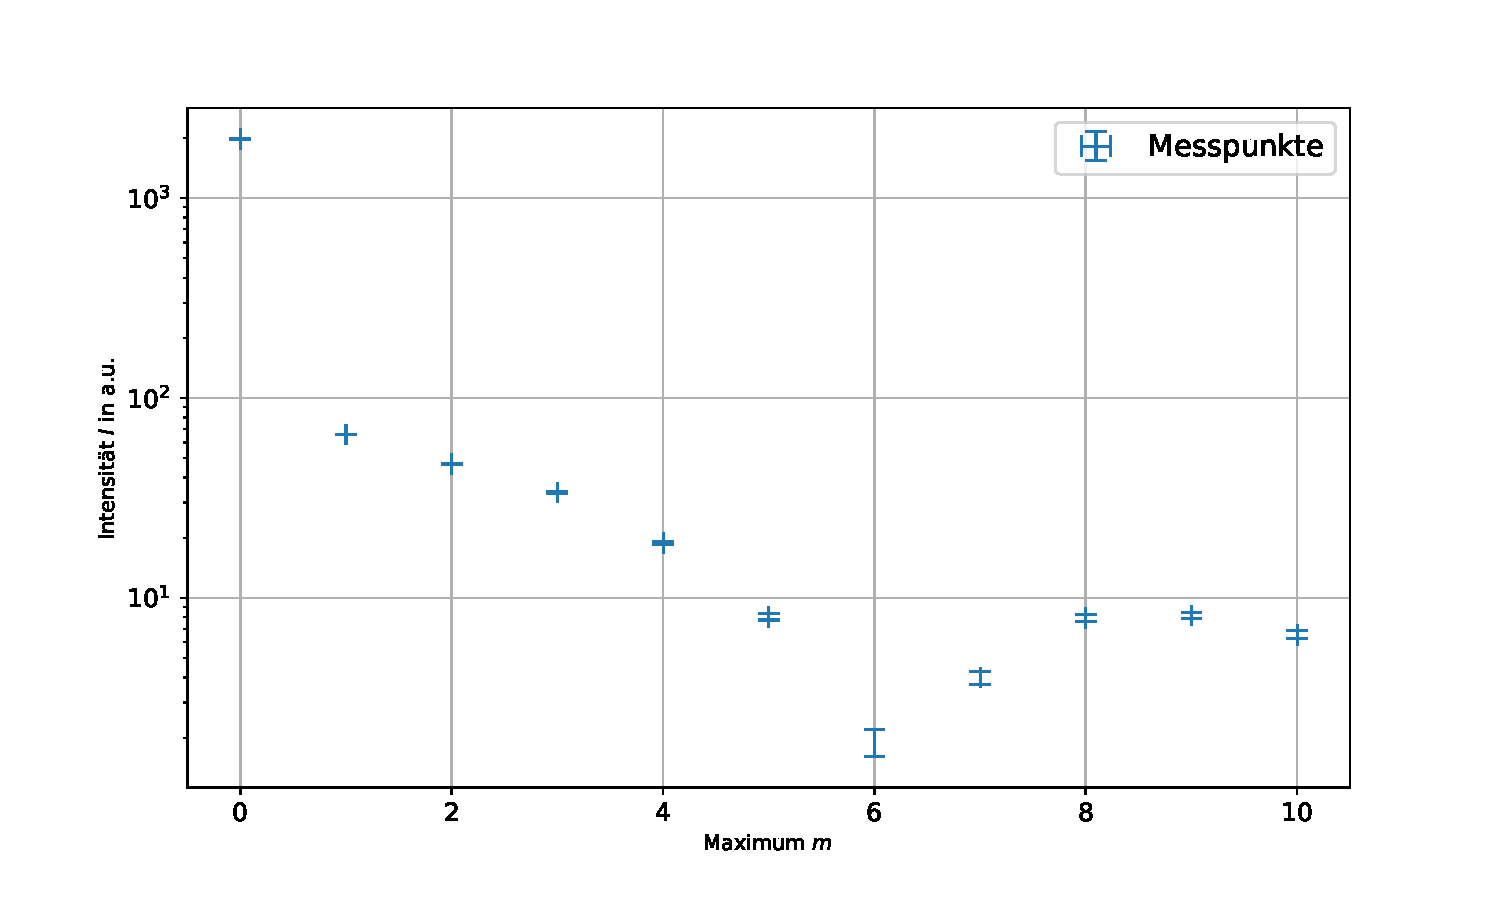
\includegraphics[width=0.8\linewidth]{img/sinc2}
			\caption{
			Messung der Intensität in Maxima der Gitterbeugung in horizontaler Richtung.
			}
			\label{fig_sinc2}
	\end{figure}


			\subsubsection*{Diskussion}
			%TODO Warum Untermodulation?

		\subsection{Beugungsbilder verschiedener DOEs}
		%4.2.3
		%TODO Bilder
		%TODO Beugungswirkungsgrad bestimmen


		%TODO Beobachtung, Änderung mit Strukturgröße
			\subsubsection*{Diskussion}
			%TODO Warum kann ein LC-Modulator Beugungsbilder erzeugen?

		\subsection{Brennweite eines Fesnel-Linsen-DOEs}
		%4.3.1
		%TODO Brennweite gegen Linsenphase auftragen

			\subsubsection*{Diskussion}
			%TODO die Anleitung klingt so, als würden sich da mehrere Fokuspositionen ergebn, aber das kann ja wohl nicht sein.
			%TODO auftretende Proportionalität beschreiben
			%TODO feststellen: Computergesteuerte Hologramme können als Linsen verschiedener Brennweite agieren.


		\subsection{Verschiedene DOEs als Hologramme}
		%4.3.2, 4.3.3
		%TODO Bilder

			\subsubsection*{Diskussion}
			%TODO DOEs nebeneinander: qualitativ Beugungsbild beschreiben, zugrundeliegenden physikalischen Effekte beschreiben
			%TODO Glas-Hologrammfrage beantworten

	\section{Schlussfolgerung}
	% Rückgriff auf Hypothese und drittes Nennen dieser

	% Quellen zitieren, Websiten mit Zugriffsdatum
	% Verweise auf das Laborbuch (sind erlaubt)
	% Tabelle + Bilder mit Beschriftung
	%\printbibliography
\end{document}

%TODO vlt die Diskussionssections alle mit * machen, weil das im Inhaltsverzeichnis wenig hilfreich ist.
